% ==============================================================================
% CHAPTER 3 — Classification: Logistic Regression, k-NN, Naive Bayes
% ==============================================================================
\chapter{Classification --- Logistic Regression, k-NN, Naive Bayes}\label{ch:classification}

\begin{intuition}[title=\textbf{Chapter Overview}]
Classification assigns discrete labels to inputs. This chapter covers three foundational classifiers---logistic regression (a discriminative probabilistic model), $k$-nearest neighbours (a non-parametric method), and Naive Bayes (a generative model)---together with the evaluation metrics needed to compare them.
\end{intuition}

% ==============================================================================
\section{Logistic Regression}
% ==============================================================================

\subsection{The Sigmoid Function and Model Formulation}

\begin{definition}[Logistic / Sigmoid Function]
The sigmoid function $\sigma : \R \to (0,1)$ is defined by
\[
    \sigma(z) = \frac{1}{1 + e^{-z}},
    \qquad \sigma'(z) = \sigma(z)(1 - \sigma(z)).
\]
\end{definition}

\begin{proposition}[Symmetry Property]
The sigmoid satisfies $\sigma(-z) = 1 - \sigma(z)$ for all $z \in \R$. Consequently, the function is symmetric about the point $\bigl(0, \tfrac{1}{2}\bigr)$.
\end{proposition}

\begin{definition}[Binary Logistic Model]
For $y \in \{0, 1\}$ and feature vector $\bm{x} \in \R^p$:
\[
    P(Y=1 \mid \bm{x}; \bm{\beta})
    = \sigma(\bm{\beta}^\top \bm{x})
    = \frac{1}{1 + \exp(-\bm{\beta}^\top \bm{x})},
\]
where $\bm{x}$ includes a constant $1$ for the intercept. Equivalently, the log-odds (logit) are linear:
\[
    \log\frac{P(Y=1|\bm{x})}{P(Y=0|\bm{x})} = \bm{\beta}^\top\bm{x}.
\]
\end{definition}

\begin{remark}
Unlike linear regression, logistic regression does not model $y$ directly but the \emph{probability} that $y = 1$. The sigmoid ensures outputs lie in $(0,1)$. A unit increase in $x_j$ multiplies the odds by $e^{\beta_j}$.
\end{remark}

\subsection{Maximum Likelihood Estimation}

\begin{theorem}[Log-Likelihood for Logistic Regression]
Given $\{(\bm{x}_i, y_i)\}_{i=1}^{n}$ with $y_i \in \{0,1\}$, the log-likelihood is
\[
    \ell(\bm{\beta})
    = \sum_{i=1}^{n} \bigl[y_i \log \sigma(\bm{\beta}^\top\bm{x}_i)
    + (1 - y_i)\log(1 - \sigma(\bm{\beta}^\top\bm{x}_i))\bigr].
\]
This function is concave, so any local maximum is global.
\end{theorem}

\begin{proof}
Since $y_i \sim \text{Bernoulli}(\sigma(\bm{\beta}^\top\bm{x}_i))$, the likelihood is $\prod_i \sigma_i^{y_i}(1-\sigma_i)^{1-y_i}$. Taking the logarithm gives the stated expression. Concavity follows from the Hessian $\nabla^2 \ell = -\bm{X}^\top \bm{W}\bm{X}$ where $\bm{W} = \text{diag}(\sigma_i(1-\sigma_i)) \succ 0$, hence $\nabla^2 \ell \preceq 0$.
\end{proof}

\begin{definition}[Binary Cross-Entropy Loss]
Minimising the negative log-likelihood defines the cross-entropy loss:
\[
    J(\bm{\beta}) = -\frac{1}{n}\sum_{i=1}^{n}\bigl[y_i\log\hat{p}_i + (1-y_i)\log(1-\hat{p}_i)\bigr],
    \qquad \hat{p}_i = \sigma(\bm{\beta}^\top\bm{x}_i).
\]
\end{definition}

\subsection{Gradient and Update Rule}

\begin{proposition}[Gradient of the Cross-Entropy]
\[
    \nabla_{\bm{\beta}} J = \frac{1}{n}\sum_{i=1}^{n}(\hat{p}_i - y_i)\,\bm{x}_i
    = \frac{1}{n}\bm{X}^\top(\hat{\bm{p}} - \bm{y}).
\]
This has the same form as the linear regression gradient, but with $\hat{\bm{p}} = \sigma(\bm{X}\bm{\beta})$ instead of $\bm{X}\bm{\beta}$.
\end{proposition}

\begin{algorithme}[title=\textbf{Gradient Descent for Logistic Regression}]
\begin{enumerate}
    \item Initialise $\bm{\beta}^{(0)} = \bm{0}$.
    \item At iteration $t$: compute $\hat{\bm{p}} = \sigma(\bm{X}\bm{\beta}^{(t)})$.
    \item Gradient: $\bm{g} = \frac{1}{n}\bm{X}^\top(\hat{\bm{p}} - \bm{y})$.
    \item Update: $\bm{\beta}^{(t+1)} = \bm{\beta}^{(t)} - \eta\,\bm{g}$.
    \item Repeat until convergence ($\norm{\bm{g}} < \epsilon$ or max iterations).
\end{enumerate}
\end{algorithme}

\begin{remark}
Newton's method (IRLS) converges faster by using the Hessian:
\[
    \bm{\beta}^{(t+1)} = \bm{\beta}^{(t)} + (\bm{X}^\top\bm{W}^{(t)}\bm{X})^{-1}\bm{X}^\top(\bm{y}-\hat{\bm{p}}^{(t)}),
\]
where $\bm{W}^{(t)} = \text{diag}(\hat{p}_i^{(t)}(1-\hat{p}_i^{(t)}))$. This typically converges in 5--10 iterations but costs $O(p^2 n + p^3)$ per step.
\end{remark}

\subsection{Softmax Multiclass Extension}

\begin{definition}[Softmax Regression]
For $K$ classes, define $K$ weight vectors $\bm{\beta}_1,\ldots,\bm{\beta}_K$. The probability of class $k$ is
\[
    P(Y = k \mid \bm{x}) = \frac{\exp(\bm{\beta}_k^\top \bm{x})}{\sum_{j=1}^{K}\exp(\bm{\beta}_j^\top \bm{x})}.
\]
The loss is the multiclass cross-entropy:
\[
    J = -\frac{1}{n}\sum_{i=1}^{n}\sum_{k=1}^{K} \ind\{y_i = k\}\log P(Y=k\mid\bm{x}_i).
\]
\end{definition}

\begin{proposition}[Softmax Gradient]
The gradient with respect to weight vector $\bm{\beta}_k$ is
\[
    \nabla_{\bm{\beta}_k} J = \frac{1}{n}\sum_{i=1}^{n}(P(Y=k|\bm{x}_i) - \ind\{y_i=k\})\,\bm{x}_i.
\]
\end{proposition}

% ==============================================================================
\section{$k$-Nearest Neighbours}
% ==============================================================================

\begin{definition}[$k$-NN Classifier]
Given a query point $\bm{x}_0$, let $\mathcal{N}_k(\bm{x}_0)$ denote its $k$ nearest neighbours in the training set (under a chosen distance, typically Euclidean). The predicted class is
\[
    \hat{y} = \argmax_{c}\;\sum_{i \in \mathcal{N}_k(\bm{x}_0)} \ind\{y_i = c\}.
\]
\end{definition}

\begin{definition}[Common Distance Metrics]
\begin{itemize}
    \item \textbf{Euclidean:} $d(\bm{x},\bm{x}') = \norm{\bm{x}-\bm{x}'}_2 = \sqrt{\sum_j(x_j-x_j')^2}$.
    \item \textbf{Manhattan:} $d(\bm{x},\bm{x}') = \norm{\bm{x}-\bm{x}'}_1 = \sum_j |x_j-x_j'|$.
    \item \textbf{Minkowski:} $d(\bm{x},\bm{x}') = \norm{\bm{x}-\bm{x}'}_p = \bigl(\sum_j |x_j-x_j'|^p\bigr)^{1/p}$.
\end{itemize}
\end{definition}

\begin{proposition}[Asymptotic Optimality]
As $n \to \infty$ and $k/n \to 0$ with $k \to \infty$, the $k$-NN classifier converges to the Bayes-optimal classifier. For $k=1$, the asymptotic error rate is at most twice the Bayes error.
\end{proposition}

\begin{warning}[title=\textbf{Curse of Dimensionality}]
In high dimensions, distances concentrate: for $\bm{x} \sim \mathcal{U}([0,1]^p)$, the ratio of the distance to the nearest neighbour to the farthest neighbour tends to $1$ as $p \to \infty$. This makes $k$-NN unreliable without dimensionality reduction. Feature scaling is critical.
\end{warning}

\begin{bestpractice}[title=\textbf{Choosing $k$}]
\begin{itemize}
    \item Small $k$ (e.g.\ $k=1$): low bias, high variance (noisy boundaries).
    \item Large $k$: high bias, low variance (smooth boundaries).
    \item Use odd $k$ for binary classification to avoid ties.
    \item Select $k$ via cross-validation, typically $k \in \{3, 5, 7, \ldots\}$.
    \item $k$-NN has no training phase (lazy learner), but prediction costs $O(np)$ per query (or $O(p\log n)$ with KD-trees).
\end{itemize}
\end{bestpractice}

% ==============================================================================
\section{Naive Bayes}
% ==============================================================================

\begin{definition}[Naive Bayes Classifier]
Applying Bayes' theorem with the conditional independence assumption $P(\bm{x}\mid y) = \prod_{j=1}^{p} P(x_j \mid y)$:
\[
    \hat{y} = \argmax_{c}\; P(Y=c)\prod_{j=1}^{p}P(x_j \mid Y=c).
\]
\end{definition}

\begin{remark}
The ``naive'' independence assumption is rarely true, yet Naive Bayes often performs surprisingly well. This is because classification only requires the correct \emph{ranking} of posterior probabilities, not their exact values. Even if $P(Y=c|\bm{x})$ is poorly estimated, the $\argmax$ may still be correct.
\end{remark}

\subsection{Gaussian Naive Bayes}

\begin{theorem}[Gaussian NB Decision Rule]
Assume $X_j \mid Y=c \;\sim\; \mathcal{N}(\mu_{jc},\,\sigma_{jc}^2)$. The log-posterior (up to a constant) is
\[
    \log P(Y=c\mid\bm{x})
    \propto \log\pi_c - \sum_{j=1}^{p}\left[\frac{(x_j - \mu_{jc})^2}{2\sigma_{jc}^2} + \log\sigma_{jc}\right],
\]
where $\pi_c = P(Y=c)$ is the class prior. Maximum likelihood estimates are $\hat{\mu}_{jc} = \frac{1}{n_c}\sum_{i:y_i=c}x_{ij}$ and $\hat{\sigma}_{jc}^2 = \frac{1}{n_c}\sum_{i:y_i=c}(x_{ij}-\hat{\mu}_{jc})^2$.
\end{theorem}

\begin{proof}
By Bayes' theorem, $P(Y=c|\bm{x}) \propto P(Y=c)\prod_j P(x_j|Y=c)$. Taking logarithms and substituting the Gaussian density $\frac{1}{\sqrt{2\pi}\sigma_{jc}}\exp\!\bigl(-\frac{(x_j-\mu_{jc})^2}{2\sigma_{jc}^2}\bigr)$ for each factor, then dropping terms constant across classes, yields the stated discriminant function.
\end{proof}

\begin{proposition}[Linear vs.\ Quadratic Boundaries]
When all $\sigma_{jc}$ are equal across classes, the Gaussian NB decision boundary is linear (equivalent to LDA under independence). Unequal variances yield quadratic boundaries, analogous to QDA.
\end{proposition}

\subsection{Other Naive Bayes Variants}

\begin{definition}[Multinomial and Bernoulli NB]
\begin{itemize}
    \item \textbf{Multinomial NB:} for count data (e.g.\ word frequencies in text). Assumes $P(\bm{x}|Y=c) \propto \prod_j \theta_{jc}^{x_j}$.
    \item \textbf{Bernoulli NB:} for binary features. Assumes $P(x_j|Y=c) = \theta_{jc}^{x_j}(1-\theta_{jc})^{1-x_j}$.
\end{itemize}
Laplace smoothing ($\alpha=1$) prevents zero probabilities: $\hat{\theta}_{jc} = \frac{n_{jc}+\alpha}{n_c + \alpha V}$ where $V$ is the vocabulary size.
\end{definition}

% ==============================================================================
\section{Decision Boundaries}
% ==============================================================================

\begin{center}
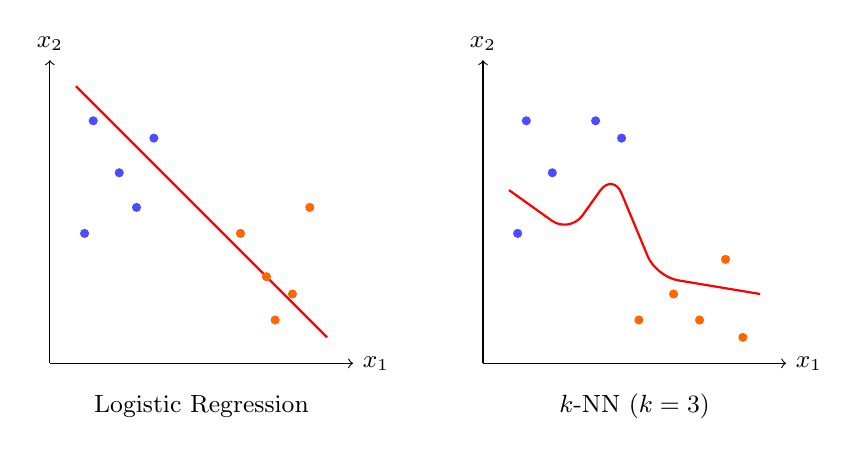
\begin{tikzpicture}[scale=1.1]
    % Logistic boundary (linear)
    \begin{scope}
        \draw[->] (0,0) -- (3.5,0) node[right] {\small $x_1$};
        \draw[->] (0,0) -- (0,3.5) node[above] {\small $x_2$};
        \draw[thick, red] (0.3,3.2) -- (3.2,0.3);
        \foreach \x/\y in {0.5/2.8, 0.8/2.2, 1.0/1.8, 0.4/1.5, 1.2/2.6}{
            \fill[blue!70] (\x,\y) circle (1.5pt);
        }
        \foreach \x/\y in {2.5/1.0, 2.8/0.8, 2.2/1.5, 3.0/1.8, 2.6/0.5}{
            \fill[orange!80!red] (\x,\y) circle (1.5pt);
        }
        \node at (1.75,-0.5) {\small Logistic Regression};
    \end{scope}
    % k-NN boundary (non-linear)
    \begin{scope}[xshift=5cm]
        \draw[->] (0,0) -- (3.5,0) node[right] {\small $x_1$};
        \draw[->] (0,0) -- (0,3.5) node[above] {\small $x_2$};
        \draw[thick, red, rounded corners=8pt]
            (0.3,2.0) -- (1.0,1.5) -- (1.5,2.2) -- (2.0,1.0) -- (3.2,0.8);
        \foreach \x/\y in {0.5/2.8, 0.8/2.2, 1.3/2.8, 0.4/1.5, 1.6/2.6}{
            \fill[blue!70] (\x,\y) circle (1.5pt);
        }
        \foreach \x/\y in {2.5/0.5, 2.8/1.2, 2.2/0.8, 1.8/0.5, 3.0/0.3}{
            \fill[orange!80!red] (\x,\y) circle (1.5pt);
        }
        \node at (1.75,-0.5) {\small $k$-NN ($k=3$)};
    \end{scope}
\end{tikzpicture}
\end{center}

% ==============================================================================
\section{Evaluation Metrics}
% ==============================================================================

\begin{definition}[Confusion Matrix]
For a binary classifier with predictions $\hat{y}_i$ and true labels $y_i$:
\[
\renewcommand{\arraystretch}{1.3}
\begin{array}{c|cc}
     & \hat{y}=1 & \hat{y}=0 \\\hline
     y=1 & \text{TP} & \text{FN} \\
     y=0 & \text{FP} & \text{TN}
\end{array}
\]
\end{definition}

\begin{definition}[Precision, Recall, F1-Score]
\[
    \text{Precision} = \frac{\text{TP}}{\text{TP}+\text{FP}},
    \qquad
    \text{Recall} = \frac{\text{TP}}{\text{TP}+\text{FN}},
    \qquad
    F_1 = \frac{2 \cdot \text{Prec} \cdot \text{Rec}}{\text{Prec}+\text{Rec}}.
\]
\end{definition}

\begin{proposition}[F-beta Score]
The general $F_\beta$ score weights recall $\beta$ times more than precision:
\[
    F_\beta = (1+\beta^2)\frac{\text{Prec}\cdot\text{Rec}}{\beta^2\cdot\text{Prec}+\text{Rec}}.
\]
$F_2$ emphasises recall (useful when missing positives is costly); $F_{0.5}$ emphasises precision.
\end{proposition}

\begin{definition}[ROC Curve and AUC]
The \emph{Receiver Operating Characteristic} (ROC) curve plots the True Positive Rate (Recall) against the False Positive Rate $\text{FPR} = \frac{\text{FP}}{\text{FP}+\text{TN}}$ as the classification threshold varies from $0$ to $1$. The \emph{Area Under the Curve} (AUC) summarises discriminative power:
\[
    \text{AUC} = P(\hat{p}_{Y=1} > \hat{p}_{Y=0}),
\]
i.e., the probability that a randomly chosen positive is scored higher than a randomly chosen negative.
\end{definition}

\begin{proposition}[AUC Interpretation]
$\text{AUC} = 0.5$ corresponds to a random classifier, $\text{AUC} = 1.0$ to a perfect classifier. AUC is invariant to the classification threshold and to class prevalence. For imbalanced datasets, the \emph{precision--recall AUC} (PR-AUC) is often more informative.
\end{proposition}

\begin{warning}[title=\textbf{Accuracy Is Not Enough}]
On imbalanced datasets (e.g.\ 95\% negatives), a classifier that always predicts negative achieves 95\% accuracy. Precision, recall, F1, and AUC give a more faithful picture of performance in such settings.
\end{warning}

% ==============================================================================
\section{Implementation in Python}
% ==============================================================================

\subsection{Logistic Regression from Scratch}

\begin{codeblock}[title=\textbf{Logistic Regression --- Gradient Descent}]
\begin{minted}{python}
import numpy as np

def sigmoid(z):
    return 1 / (1 + np.exp(-np.clip(z, -500, 500)))

def logistic_fit(X, y, eta=0.1, n_iter=1000):
    n, p = X.shape
    X_aug = np.column_stack([np.ones(n), X])
    beta = np.zeros(X_aug.shape[1])
    for _ in range(n_iter):
        p_hat = sigmoid(X_aug @ beta)
        grad = (1 / n) * X_aug.T @ (p_hat - y)
        beta -= eta * grad
    return beta

def logistic_predict(X, beta, threshold=0.5):
    X_aug = np.column_stack([np.ones(X.shape[0]), X])
    return (sigmoid(X_aug @ beta) >= threshold).astype(int)
\end{minted}
\end{codeblock}

\subsection{Scikit-Learn Classifiers}

\begin{codeblock}[title=\textbf{Logistic Regression, k-NN, Naive Bayes with scikit-learn}]
\begin{minted}{python}
from sklearn.datasets import load_iris
from sklearn.model_selection import train_test_split
from sklearn.preprocessing import StandardScaler
from sklearn.linear_model import LogisticRegression
from sklearn.neighbors import KNeighborsClassifier
from sklearn.naive_bayes import GaussianNB
from sklearn.metrics import (accuracy_score, classification_report,
                             roc_auc_score, confusion_matrix)

X, y = load_iris(return_X_y=True)
# Binary task: versicolor vs. virginica
mask = y != 0
X, y = X[mask], (y[mask] - 1)  # labels 0 and 1

X_train, X_test, y_train, y_test = train_test_split(
    X, y, test_size=0.3, random_state=42)
scaler = StandardScaler().fit(X_train)
X_tr = scaler.transform(X_train)
X_te = scaler.transform(X_test)

models = {
    "Logistic": LogisticRegression(max_iter=500),
    "k-NN (k=5)": KNeighborsClassifier(n_neighbors=5),
    "Gaussian NB": GaussianNB(),
}
for name, clf in models.items():
    clf.fit(X_tr, y_train)
    y_pred = clf.predict(X_te)
    acc = accuracy_score(y_test, y_pred)
    print(f"{name:15s}  Accuracy: {acc:.3f}")
\end{minted}
\end{codeblock}

\begin{codeoutput}
\begin{minted}{text}
Logistic         Accuracy: 0.967
k-NN (k=5)      Accuracy: 0.933
Gaussian NB      Accuracy: 0.967
\end{minted}
\end{codeoutput}

\begin{codeblock}[title=\textbf{ROC Curve and Confusion Matrix}]
\begin{minted}{python}
from sklearn.metrics import RocCurveDisplay, ConfusionMatrixDisplay
import matplotlib.pyplot as plt

fig, axes = plt.subplots(1, 2, figsize=(10, 4))

# ROC curve for logistic regression
lr = models["Logistic"]
RocCurveDisplay.from_estimator(lr, X_te, y_test, ax=axes[0])
axes[0].set_title("ROC Curve -- Logistic Regression")

# Confusion matrix
ConfusionMatrixDisplay.from_estimator(
    lr, X_te, y_test, ax=axes[1], cmap="Blues")
axes[1].set_title("Confusion Matrix")

plt.tight_layout()
plt.savefig("roc_cm.pdf")
\end{minted}
\end{codeblock}

\begin{codeblock}[title=\textbf{Cross-Validation for k-NN}]
\begin{minted}{python}
from sklearn.model_selection import cross_val_score
import numpy as np

k_values = [1, 3, 5, 7, 9, 15, 25]
cv_scores = []
for k in k_values:
    knn = KNeighborsClassifier(n_neighbors=k)
    scores = cross_val_score(knn, X_tr, y_train, cv=5,
                             scoring="accuracy")
    cv_scores.append(scores.mean())
    print(f"k={k:2d}: CV accuracy = {scores.mean():.3f} "
          f"(+/- {scores.std():.3f})")

best_k = k_values[np.argmax(cv_scores)]
print(f"\nBest k = {best_k}")
\end{minted}
\end{codeblock}

\begin{codeoutput}
\begin{minted}{text}
k= 1: CV accuracy = 0.914 (+/- 0.049)
k= 3: CV accuracy = 0.929 (+/- 0.048)
k= 5: CV accuracy = 0.943 (+/- 0.040)
k= 7: CV accuracy = 0.943 (+/- 0.040)
k= 9: CV accuracy = 0.929 (+/- 0.048)
k=15: CV accuracy = 0.914 (+/- 0.049)
k=25: CV accuracy = 0.900 (+/- 0.056)

Best k = 5
\end{minted}
\end{codeoutput}

% ==============================================================================
\section{Exercises}
% ==============================================================================

\begin{exercise}[Sigmoid Properties]
Prove that $\sigma(-z) = 1 - \sigma(z)$ and that $\sigma'(z) = \sigma(z)(1-\sigma(z))$. Derive the Hessian of the binary cross-entropy and show it is positive semi-definite.
\end{exercise}

\begin{exercise}[Decision Boundary Geometry]
For a binary logistic regression with two features $(x_1,x_2)$, show that the decision boundary $\{x : P(Y=1|\bm{x})=0.5\}$ is a line in $\R^2$. What determines its slope and intercept?
\end{exercise}

\begin{exercise}[$k$-NN Experiments]
Using the \texttt{make\_moons} dataset from scikit-learn:
\begin{enumerate}
    \item Fit $k$-NN for $k \in \{1, 3, 5, 15, 50\}$ and plot decision boundaries.
    \item Report 5-fold cross-validation accuracy for each $k$.
    \item Discuss the bias--variance trade-off as $k$ varies.
\end{enumerate}
\end{exercise}

\begin{exercise}[Naive Bayes Independence Assumption]
Consider two features $X_1, X_2$ with $\Cov(X_1,X_2|Y=c) \neq 0$. Explain why Gaussian NB may still perform well in practice despite the violated independence assumption. Under what conditions does it fail?
\end{exercise}

\begin{exercise}[Multiclass Softmax]
Derive the gradient $\nabla_{\bm{\beta}_k} J$ of the multiclass cross-entropy for softmax regression. Implement softmax regression from scratch on the Iris dataset (3 classes) and compare with \texttt{LogisticRegression(multi\_class='multinomial')}.
\end{exercise}

\begin{exercise}[ROC Analysis]
On a dataset of your choice, train logistic regression and Gaussian NB. Plot both ROC curves on the same axes and compare AUC scores. When does Naive Bayes outperform logistic regression?
\end{exercise}

\begin{exercise}[Regularized Logistic Regression]
scikit-learn's \texttt{LogisticRegression} applies L2 regularization by default (parameter \texttt{C} = inverse strength). Using the breast cancer dataset, plot test accuracy as a function of $C \in \{10^{-3}, 10^{-2}, \ldots, 10^{3}\}$. Which $C$ gives the best performance? Why is regularization important in logistic regression?
\end{exercise}

\begin{keyformulas}[title=\textbf{Chapter 3 Summary}]
\begin{itemize}
    \item \textbf{Logistic:} $P(Y\!=\!1|\bm{x}) = \sigma(\bm{\beta}^\top\bm{x}),\quad \nabla J = \frac{1}{n}\bm{X}^\top(\hat{\bm{p}}-\bm{y})$
    \item \textbf{Softmax:} $P(Y\!=\!k|\bm{x}) = \frac{\exp(\bm{\beta}_k^\top\bm{x})}{\sum_j \exp(\bm{\beta}_j^\top\bm{x})}$
    \item \textbf{$k$-NN:} $\hat{y} = \argmax_c \sum_{i \in \mathcal{N}_k} \ind\{y_i=c\}$
    \item \textbf{Gaussian NB:} $\hat{y} = \argmax_c \log\pi_c - \sum_j \frac{(x_j-\mu_{jc})^2}{2\sigma_{jc}^2}$
    \item \textbf{F1:} $\frac{2\cdot\text{Prec}\cdot\text{Rec}}{\text{Prec}+\text{Rec}},\quad$ \textbf{AUC:} area under ROC curve
\end{itemize}
\end{keyformulas}
